\documentclass[12pt,a4paper,final]{report}
\usepackage[english]{babel}
\usepackage[fleqn]{amsmath}
\usepackage{amsfonts}
\usepackage{amssymb}
\usepackage{mathptmx}
\usepackage{fancyhdr}
\usepackage{graphicx}
\usepackage{array}

\usepackage[%
    a4paper,
%   includeheadfoot,
    head=0.762cm,  % distance from bottom of header to block of text aka \headsep e.g. \baselineskip
    foot=0.762cm,  % distance from top of footer to block of text aka \footskip
    headheight=12pt,     % height for the header block (no equivalent for footer)
%   heightrounded,       % ensure an integer number of lines
    marginparwidth=2cm,  % right marginal note width
    marginparsep=2mm,    % distance from text block to marginal note box
%   height=\textheight,  % height of the text block
%   width=\textwidth,    % width of the text block
    top=1.7cm,           % distance of the text block from the top of the page
    bottom=1.4cm,
    left=1.9cm,
    right=1.9cm,
%    showframe,           % show the main blocks
%    verbose,             % show the values of the parameters in the log file
]{geometry}

\pagestyle{fancy}
\fancyhf{}
\rhead{\bfseries {\nouppercase{\leftmark}}}
\lhead{\bfseries DDoS Detection in Software Defined Network}
\cfoot{\bfseries \thepage}

\usepackage[table]{xcolor}
\newcolumntype{P}[1]{>{\centering\arraybackslash}p{#1}}
\newcolumntype{M}[1]{>{\centering\arraybackslash}m{#1}}

\renewcommand{\footrulewidth}{0.4pt}

\title{Detection of DDoS in SDN environment using SVM and Entropy based discretization.}
\graphicspath{ {Images/} }

\usepackage{tikz}
\usetikzlibrary{calc}
\usepackage{eso-pic}

\usepackage{titlesec}
\titleformat{\section}[block]
  {\fontsize{16}{18}\bfseries}
  {\thesection}
  {1em}
  {}
\titleformat{\subsection}[block]
  {\fontsize{14}{15}\bfseries}
  {\thesubsection}
  {1em}
  {}

\usepackage{blindtext}
\usepackage{tocloft}
\renewcommand{\cfttoctitlefont}{\hspace*{\fill}\Huge\bfseries}
\renewcommand{\cftaftertoctitle}{\hspace*{\fill}}
\renewcommand{\cftlottitlefont}{\hspace*{\fill}\Huge\bfseries}
\renewcommand{\cftafterlottitle}{\hspace*{\fill}}
\renewcommand{\cftloftitlefont}{\hspace*{\fill}\Huge\bfseries}
\renewcommand{\cftafterloftitle}{\hspace*{\fill}}

\newcommand{\abbrlabel}[1]{\makebox[6cm][l]{\textbf{#1}\ \dotfill}}
\newenvironment{abbreviations}{\begin{list}{}{\renewcommand{\makelabel}{\abbrlabel}}}{\end{list}}

\DeclareRobustCommand{\gobblefive}[5]{}
\newcommand*{\SkipTocEntry}{\addtocontents{toc}{\gobblefive}}

\usepackage{hyperref}
\hypersetup{
    colorlinks=true,
    linkcolor=black,
    citecolor=black,
}

\begin{document}
\begin{center}
\thispagestyle{empty}
\vspace*{1cm}
A PRELIMINARY PROJECT REPORT
\vspace*{0.75cm}

ON
\vspace*{0.75cm}

\Large
DETECTION OF DDoS IN SDN ENVIRONMENT USING SVM AND ENTROPY  BASED DISCRETIZATION.
\vspace*{0.75cm}

\normalsize
\begin{figure}[h]
\begin{center}

\includegraphics[width=5.5cm, height=6cm]{logo.png}
\end{center}
\end{figure}

\vspace*{0.5cm}
BY
\vspace*{0.35cm}
\linebreak
ACHYUTH RAO
\linebreak
AKIB SHAIKH
\linebreak
ARUN POTTEKAT
\linebreak
PRANAV TALE
\linebreak

\large
\vspace*{0.5cm}
DEPARTMENT OF COMPUTER ENGINEERING
\linebreak
P.E.S MODERN COLLEGE OF ENGINEERING
\linebreak
PUNE - 411005.
\linebreak
$[$ 2016 – 2017 $]$
\end{center}
\newpage

\thispagestyle{empty}
\vspace*{60px}
\underline{\hspace{16cm}}
\vspace*{30px}

\begin{center}
\textbf{A PRELIMINARY PROJECT REPORT}\\

\vspace*{25px}
\textbf{ON}

\vspace*{25px}

\begin{huge}
\textbf{``Detection of DDoS in SDN Environment using SVM and Entropy based discretization''}\par
\end{huge}

\vspace*{13px}
\textbf{Version: 1.0, \today}

\vspace*{40px}
\textbf{By}\\

\vspace*{30px}
\textbf{Achyuth Rao}\\
\textbf{Akib Shaikh}\\
\textbf{Arun Pottekat}\\
\textbf{Pranav Tale}

\end{center}

\vspace*{5cm}
\underline{\hspace{16cm}}
\newpage

\thispagestyle{empty}
\vspace*{7cm}

\textbf{Guide:}

\begin{itemize}
\addtolength{\itemindent}{.5cm}
\item \textbf{Internal Guide Name:} Ms. Aparna Junnarkar

\end{itemize}

\vspace{1cm}

\textbf{Presented By:}

\begin{center}

\begin{tabular}{|>{\bf}m{3.5cm}|>{\bf}m{3.5cm}|>{\bf}m{3.5cm}|>{\bf}m{3.5cm}|}
\hline
\rowcolor{lightgray}
Date & Version & Title & Authors \\
\hline
\normalfont{$6^{th}$ October, 2016} & 
\normalfont{1.0} & 
\normalfont{Detection of DDoS in SDN Environment using SVM and Entropy based discretization} & 
\normalfont{Achyuth Rao, Akib Shaikh, Arun Pottekat, Pranav Tale}\\
\hline
\end{tabular}

\end{center}
\newpage

\thispagestyle{empty}
\vspace*{1.3cm}
\begin{center}

\includegraphics[width=5.5cm, height=6cm]{logo.png}
\end{center}
\begin{center}
\Large
Progressive Education Society's \\
\textbf{Modern College of Engineering} \\
Shivajinagar, Pune - 411005. \\
\vspace{1cm}

\underline{\textbf{CERTIFICATE}}
\end{center}
\normalsize
\vspace{0.5cm}
This is to certify that the following students of Final Year Computer Engineering have successfully completed the preliminary analysis and design of project entitled ``Detection of DDoS in SDN environment using SVM and Entropy based mechanism'' for the organization ``PES Modern College Of Engineering'' \\
The Group Members names are: \hspace{0.1cm} Sandhyavandanam Achyuth Rao. \\\hspace*{5.7cm} Akib Ashraf Shaikh. \\
\hspace*{5.7cm} Arun Pramod Pottekat. \\
\hspace*{5.7cm} Pranav Balasaheb Tale. \vspace{1cm}\\
This is in partial fulfillment of Bachelor of Computer Engineering under Savitribai Phule Pune University. \vspace{1cm}\\
Date: \vspace{2cm} \\
\hspace*{0.8cm}Internal Guide 	 
\hspace{3.95cm}Head Of Dept
\hspace{3.5cm}External Examiner \\
(Ms. Aparna Junnarkar)
\hspace*{2.3cm}(Computer Engineering) \\
\hspace*{6.3cm}(Dr. Prof. Mrs. S. A. Itkar) \\

\thispagestyle{empty}
\Large
\begin{center}
\chapter*{\centering Acknowledgement}
\end{center}
\normalsize
It gives us pleasure in presenting the preliminary project report on \textbf{`Detection of Distributed Denial of service attack in Software Defined Network using Support Vector Machine and Entropy Based Discretization'}.\\

Firstly, we would like to express our indebtedness appreciation to our internal guide \textbf{Ms. Aparna A. Junnarkar}. Her constant guidance and advice played very important role in making the execution of the report. She always gave us her suggestions, that were crucial in making this report as flawless as possible.\\

We would like to express our gratitude towards \textbf{Prof. Dr. Mrs. S. A. Itkar}  Head of Computer Engineering Department, PES Modern College of Engineering for her kind co-operation and encouragement which helped us during the completion of this report.\\

Also, we would like to thank \textbf{Mr. Kunal Khadke, Ms. Yogita Narwadkar, Mr. B. D. Phulpagare, Ms. Pallavi Baviskar, Ms. Deipali V. Gore, Ms. Renuka Kajale} and all \textbf{Technical assistants} for providing time to time guidance and various resources such as laboratory with all needed software platforms and continuous Internet connection for our Project.\\

In the end special thanks to all our classmates for helping us out during the entire documentation process.

\begin{flushright}
Achyuth Rao\\
Akib Shaikh\\
Arun Pottekat\\
Pranav Tale\\
\end{flushright}
\newpage

\pagestyle{plain} 
\cleardoublepage
\pagenumbering{gobble}
\tableofcontents
\newpage

\pagenumbering{roman}
\Large
\chapter*{\centering Abstract}
\addcontentsline{toc}{chapter}{Abstract}
\normalsize
\noindent
The current networking paradigm involves switches, routers and gateways where these networking devices constitute both logical thinking as well as routing of packets. Traditionally the network administrator is responsible for configuring and managing these devices manually and at all times, which makes it a tedious task. 

With the onset of the Software Defined Network, this task of manually managing the devices reduces to some extent, as it seperates the control plane from the data plane i.e. Forwarding of
packets is done in the data plane and intelligence of the entire network resides in the control plane. 

Data plane constitutes the network devices which comprise switches known as "dumb terminals" and the control plane constitutes a central controller which keeps track of all switches in the network.

Due to the centralized nature of SDN i.e. the controller at the center of SDN taking the logical decisions, there arises a threat of malicious users launching cyber attacks on this central component thereby, dislodging the entire network. Some attacks include Application level attacks, Brute Force attack, man in the middle attacks, DDoS attack etc.

Distributed Denial of Service attack involves a single malicious user controlling different users known as bots to launch an attack
against a single entity in the network without even the victim being aware of the attack. DDoS attacks result in direct financial losses along with damage to company reputation and loss of the customer's trust.

As a part of solution to this problem, two algorithms can be used for the detection of DDoS attack i.e. Support Vector Machine, a machine learning algorithm and Entropy based Discretization, a Data Mining algorithm.

Support Vector Machine takes the rate of incoming packets as the input and classifies them as normal traffic or attack traffic. Whereas Entropy based Discretization monitors the entropy of the network i.e. measure of randomness and if it falls below a threshold value then it is classified as attack traffic.

Once the attack is detected by either of the applications, an entry will be made in the log files  constantly monitored by network monitoring tools and thus report the incident back to the network adminstrative team. 

The network adminstrator would be provided a monitoring application which would display the details of the attack detected such as the source IP and victim IP etc.

As a part of the project, comparison studies will also be done related to both algorithms displaying the rate at which attacks are detected along with their accuracies.
\newpage

\listoffigures
\addcontentsline{toc}{chapter}{List of Figures}
\newpage
\listoftables
\addcontentsline{toc}{chapter}{List of Tables}
\newpage

\chapter*{\centering List of Abbreviations}
\begin{abbreviations}
\item[SDN] Software Defined Network
\item[SVM] Support Vector Machine
\item[DDoS] Distributed Denial of Service
\item[ONOS] Open Network Operating Switch
\item[OVSDB] Open vSwitch Database
\item[EBD] Entropy based Discretization
\item[NP] Non Polynomial Time
\item[P] Polynomial Time
\item[HTTP] Hyper Text Transfer Protocol
\item[UDP] Uniform Datagram Protocol
\item[TCP] Transmission Control Protocol
\item[k-NN] K Nearest Neighbour
\item[ICMP] Internet Control Message Protocol
\item[FTP] File Transfer Protocol
\item[QP] Quadratic problem
\end{abbreviations}

\addcontentsline{toc}{chapter}{List of Abbreviations}
\newpage
\pagestyle{fancy}
 
\newcommand{\hsp}{\hspace{0pt}}
\titleformat{\chapter}[hang]
{\flushright\fontseries{b}\fontsize{80}{100}\selectfont}{\fontseries{b}\fontsize{72}{84}\selectfont\textcolor{black}\thechapter\hsp}{0pt}
{.\\ \Huge\bfseries}
[]\titlespacing*{\chapter}{0pt}{540pt}{20pt}	

\pagenumbering{gobble}
\pagenumbering{arabic}

\AddToShipoutPictureBG*{%
\begin{tikzpicture}[overlay,remember picture]
\draw[line width=1.5pt]
    ($ (current page.north west) + (0.7cm,-0.7cm) $)
    rectangle
    ($ (current page.south east) + (-0.7cm,0.7cm) $);
\draw[line width=1.5pt]
    ($ (current page.north west) + (0.9cm,-0.9cm) $)
    rectangle
    ($ (current page.south east) + (-0.9cm,0.9cm) $);
\end{tikzpicture}
}
\chapter{Software Requirement Specification}
\thispagestyle{empty}
\newpage
\section{Purpose}
The number of Cyber Attacks is increasing day by day and has become a major concern for enterprises. Such attacks include application level attack, man in the middle attack, brute force, DDoS etc. Attackers are waging an asymmetric battle against these enterprises on their networks, assets and data. One major type of attack would be Distributed Denial of Service attack which is launched by flooding the targeted machine with multiple requests to overload the system and prevent the legitimate packets. In the next generation networking, when Software Defined Networks would be deployed in data centers, enterprises or campus networks, security will prove to be a critical issue against such attacks that needs to be taken care of, which is the aim of our project.

In Software Defined Networks, the network intelligence and state are logically centralized which gives programmability, better network control, flexibility and scalability. But in this new architecture the controller which is responsible for controlling the whole network can become a single point of attack. In our proposed method, we will be using Support Vector Machine, Entropy Based Discretization as well as Fuzzy C Means clustering in order to effectively detect any DDoS attack that takes place in a Software Defined Network.

\section{Project Scope}
The scope of the project extends to setting up of a Software Defined Network using OpenFlow configured switches and also use three algorithms i.e. Entropy based discretization, Fuzzy C Means Clustering and Support Vector Machine for the detection of DDoS attacks. As a part of this project we would also be using a network monitoring tool to monitor the software defined network and raise a notification as soon as any of the three algorithms reports a DDoS attack by marking an entry into the log files which could be utilized for future needs.

\section{Usage Scenario}
\subsection{User profiles}
\begin{enumerate}
\item
\textbf{Network Administrative team :}
Every software or non-software industry now-a-days involves its own network establishment. A network administrative team is delegated the task of monitoring the network activities and troubleshooting the network in case of any issues. 
\par
Currently this team faces a tough task of manually monitoring the network for any attacks at all times.
Deployment of our product in an enterprise would reduce the burden of the network team as they would receive a notification whenever DDoS attack occurs thereby allowing them to take precautionary measures.
\end{enumerate}

\newpage
\subsection{Use-cases}
\begin{table}[h]
\begin{center}
\begin{tabular}{|p{1cm}|p{3cm}|p{4cm}|p{3.5cm}|p{4cm}|}
\hline 
\textbf{Sr. No.} & \textbf{Use Case} & \textbf{Description} & \textbf{Actors} & \textbf{Assumptions} \\ 
\hline 
1 & DDoS Notification raised & Raising DDoS notification as soon as DDoS is detected by any of the three algorithms i.e. Support Vector Machine, Entropy based discretization and Fuzzy C-Means Clustering & Network Administrator & SDN is established within the environment and DDoS attack is launched on the enterprise. \\
\hline
2 & Network Monitoring & Monitoring the network statistics for any anomalies using sFlow, ElasticSearch Logstash Kibana (ELK Stack), and Flask based application & Network administrator & The link between switches and the monitoring system is maintained throughout. \\
\hline 
\end{tabular} 
\end{center}
\caption{Use cases}
\end{table}

\subsection{Use Case Diagram}
\begin{figure}[h]
\begin{center}
\includegraphics[scale=0.5]{use_case.png}
\caption{Use Case Diagram}
\end{center}
\end{figure}

\newpage
\section{Product Features}
\begin{enumerate}
\item
\textbf{Runtime Detection of DDoS attack :-}
\newline
In the current network scenario, there aren't many utilies for efficient DDoS detection. Due to this, the network administrator has to monitor the network continuously. Hence, this product will be step towards the automation of this process wherein the network administrator will have to verify the attack, only when the notification is generated.

\item
\textbf{Network Environment Specific Product :-}
\newline
The training of the Support Vector Machine algorithm and Fuzzy C Means Clustering is done using an environment specific conditions or depending on the normal network traffic conditions in your network. Thus these algorithms are trained in such a way so as to reduce the false positive rate of detection. Also the threshold for Entropy Based mechanism is decided depending on the normal traffic conditions.

\item
\textbf{Automated Alert Mechanism :-}
\newline
As soon as the attack is generated the alert can be sent to a specific network monitoring team or can send an email along with the information of where the attack has occurred specifying the IP addresses.

\item
\textbf{Suitable for all Software Defined Networks :-}
\newline
Independent of what type of Software Defined Network like carrier, service provider, enterprise, data center or campus network, our solution will be effective in all these environments.

\item
\textbf{Open Source to encourage contribution and research :-}
\newline
As SDN itself is an open standard of next generation networking, our solution will be made open source along with the source code and the method of detection, describing the step-by-step complete procedure. This will help us to encourage the open source community to contribute their ideas and ultimately improve the effectiveness.

\item
\textbf{SDN Controller Independent :-}
\newline
Since our application will the running on the edge switches, irrespective of which SDN controller is in use our solution can still be used.
\end{enumerate}

\newpage
\section{Functional Model and Description}
\subsection{Data Flow Diagram}
\begin{enumerate}
\item
\textbf{Level 0 Data Flow Diagram :}
\newline
\begin{figure}[h]
\begin{center}
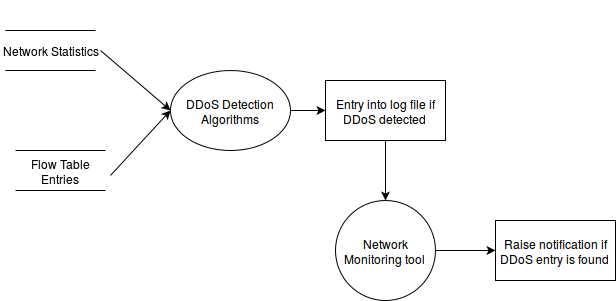
\includegraphics[scale=0.6]{dataflow0.png}
\caption{Level 0 Data Flow Diagram}
\end{center}
\end{figure}

\item
\textbf{Level 1 Data Flow Diagram :}
\newline
\begin{figure}[h]
\begin{center}
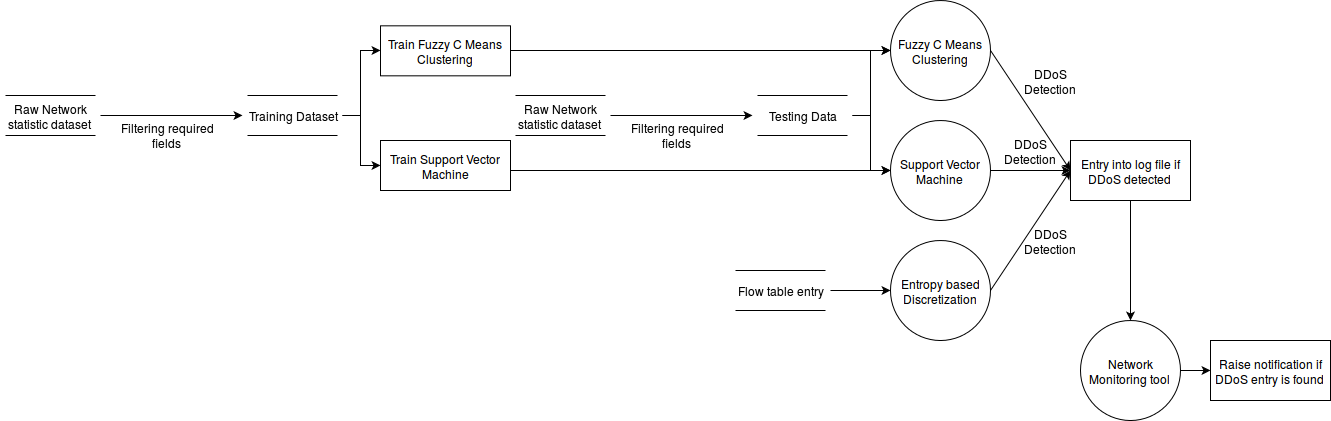
\includegraphics[scale=0.4]{dataflow1.png}
\caption{Level 1 Data Flow Diagram}
\end{center}
\end{figure}
\end{enumerate}

\newpage
\subsection{Activity Diagram}
\begin{figure}[h]
\begin{center}
\includegraphics[scale=0.5]{activity.png}
\caption{Activity Diagram}
\end{center}
\end{figure}

\subsection{Non Functional Requirements}
\begin{enumerate}
\item
\textbf{Interface Requirements}
\begin{enumerate}
\item OpenFlow Protocol :
\newline
Provides a medium for the SDN controller to direct traffic along the switches within the network.

\item Northbound API's :
\newline
Allow the SDN controller to communicate between services and applications running over the network owing to programmatic nature of SDN.

\item Southbound API's :
\newline
Allow the SDN controller to communicate between the network devices within the network.
\end{enumerate}

\item
\textbf{Software Quality Attributes}
\begin{enumerate}
\item Correctness:
\newline
The correctness of our product would depend upon the accuracy with which either of the application would detect the attack. For this purpose both applications must be trained in the network which they would monitor to generate the necessary constant values needed for their execution.

\item Availability:
\newline
As long as the network is up and running, this service would be also be available continuously monitoring the network for any anomalies.

\newpage
\item Usability: 
\newline
As and when a DDoS attack is detected, a simple notification is sent to the network administrative team. It does not disrupt their normal work flow or involve using complex application for monitoring purposes. Hence no specific training of the user is needed for using this system. 

\item Portability: 
\newline
Portability is restricted i.e. both applications must be given prior training before being deployed in a network. Thus the system being used in one enterprise cannot be used in another enterpise owing to the fact that the network traffic would vary from enterprise to enterprise such that normal traffic in one could be classified as attack traffic in another enterprise. Hence training in the network is of utmost importance.
\end{enumerate}
\end{enumerate}

\subsection{State Diagram}
\begin{figure}[h]
\begin{center}
\includegraphics[scale=0.6]{state.png}
\caption{State Diagram}
\end{center}
\end{figure}
\newpage

\AddToShipoutPictureBG*{%
\begin{tikzpicture}[overlay,remember picture]
\draw[line width=1.5pt]
    ($ (current page.north west) + (0.7cm,-0.7cm) $)
    rectangle
    ($ (current page.south east) + (-0.7cm,0.7cm) $);
\draw[line width=1.5pt]
    ($ (current page.north west) + (0.9cm,-0.9cm) $)
    rectangle
    ($ (current page.south east) + (-0.9cm,0.9cm) $);
\end{tikzpicture}
}
\chapter{Detailed Design Document}
\thispagestyle{empty}
\newpage
\section{Architectural Design}
\begin{figure}[h]
\begin{center}
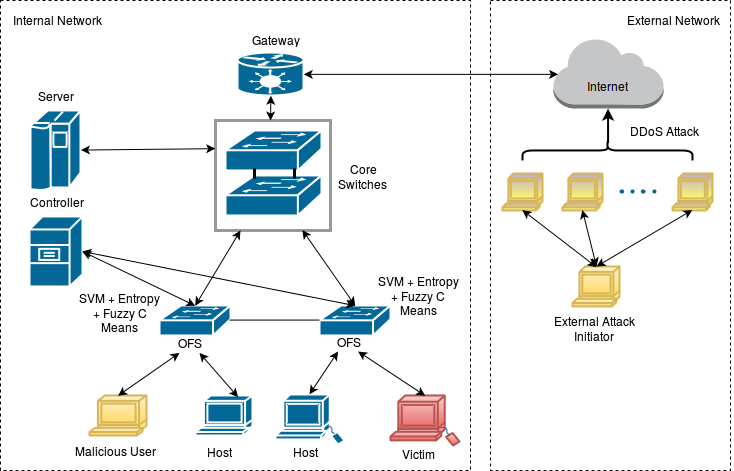
\includegraphics[scale=0.6]{architecture.png}
\caption{System Architecture}
\label{Architecture}
\end{center}
\end{figure}

During normal state of communication between two users in the network, the first packet is transmitted from the host to it's nearby switch. Initially the switch does not have any entry in its flow table as to where it should forward the incoming packet, hence the default route is to forward the packet to the controller. The controller then dictates the switch to forward the packet to the respective destination port. Along with this the controller also makes an entry in the flow table of the switch for the particular source and destination such that the future packets with the same source and destination are forwarded directly without any intervention of the controller.

This helps in reducing the time taken for communication between source and destination systems. After a particular interval of time the flow table entries are flushed and the process is repeated all over again.

The system is designed to detect two types of DDoS attacks namely :-
\begin{enumerate}
\item
Internal DDoS attack

\item
External DDoS attack
\end{enumerate}

In the first case, i.e. internal DDoS attack, the malicious user and the victim are located within the software defined network. 
whereas in external DDoS attack the host machine is from a different network. In both cases losses generated are immense.

The malicious machine can now launch attacks at two different points, one being the controller which would result in downfall of entire enterprise network incase there aren't any secondary controllers available, or the second point of attack could be one of host machines. 

In case of the attack point being the controller, the attack is generated by spoofing the source and destination ip address so that it does not match any flow table entry and hence must make a trip to the controller, this would burden the controller and thereby render its services unavailable. To overcome this issue, SVM monitors the rate of incoming packets and classifies it as normal traffic or attack traffic, similarly Entropy based mechanism would find a drop in the entropy in the network owing to the large number of same class of packets hence would be able to detect the DDoS attack, and Fuzzy C Means clustering would assign a membership value closer to "1" near the core switch since all packets are being directed towards the controller and thus would be able to detect a DDoS attack.

Another method of generating an attack would be by generating a multitude of requests at the host thereby rendering the system void of performing any other operations. This type of attack is also solved along similar guidelines such that SVM would monitor the rate of incoming packets and Entropy based mechanism would monitor the entropy of the network which would drop due to large number of same class of packets, similarly Fuzzy C Means, running on the edge switches would be able to place the incoming packets in the attack cluster thereby detecting a DDoS attack.

Hence, a comparison can be deduced as to which method would generate a result instantaneously and with higher accuracy.

Once the attack is detected by any of the applications an entry is made into the log file of the respective switch, which is constantly monitored by the network monitoring tool which on finding the entry raises a notification to the network admnistrative team. Further it is the responsibility of the network administrative team to take preventive measures to eliminate any damage that could be caused by an impending full fledged DDoS attack.

\section{Data Design}
\subsection{Dataset Description}
For the purpose of detection, all three algorithms use some form of data on which computation is performed and results are predicted. In case of Support Vector Machine the dataset consists of the network statistics, which have been converted to a "csv" file with limited fields using a terminal based tool "tshark".
\newline

The fields present in the dataset have been shown in table 2.1
\begin{table}[h]
\begin{center}
\begin{tabular}{|p{3cm}|p{3cm}|p{4cm}|p{3.5cm}|p{4cm}|}
\hline 
\textbf{Packet Interval} & \textbf{Source IP} & \textbf{Destination IP} & \textbf{Protocol} \\ 
\hline 
0.000300000 & 192.168.1.14 & 192.168.1.11 & 1 \\ 
\hline
\end{tabular} 
\end{center}
\caption{Dataset Fields - Support Vector Machine}
\end{table}

\begin{enumerate}
\item
\textbf{Packet Interval :}
\newline
Time interval between two incoming packets

\item
\textbf{Source IP :}
\newline
The source ip address of the sender machine.

\item
\textbf{Destination IP :}
\newline
The destination ip address of the receiver machine.

\item
\textbf{Protocol}
\newline
Protocol of the incoming packet.
\end{enumerate}

This dataset is again categorized into attack traffic dataset and normal traffic dataset, which can be shown in table 2.2 and 2.3, wherein the most standout variation is the packet interval field between normal traffic and attack traffic.
\begin{table}[h]
\begin{center}
\begin{tabular}{|p{3cm}|p{3cm}|p{4cm}|p{3.5cm}|p{4cm}|}
\hline 
\textbf{Packet Interval} & \textbf{Source IP} & \textbf{Destination IP} & \textbf{Protocol} \\ 
\hline 
0.000300000 & 192.168.1.14 & 192.168.1.11 & 1 \\ 
\hline
0.000100000 & 192.168.1.12 & 192.168.1.11 & 1 \\ 
\hline
0.000200000 & 192.168.1.13 & 192.168.1.11 & 6 \\ 
\hline
\end{tabular} 
\end{center}
\caption{Attack Dataset Fields - Support Vector Machine}
\end{table}

\newpage
\begin{table}[h]
\begin{center}
\begin{tabular}{|p{3cm}|p{3cm}|p{4cm}|p{3.5cm}|p{4cm}|}
\hline 
\textbf{Packet Interval} & \textbf{Source IP} & \textbf{Destination IP} & \textbf{Protocol} \\ 
\hline 
0.02000000 & 192.168.1.14 & 192.168.1.11 & 1 \\ 
\hline
0.01000000 & 192.168.1.14 & 192.168.1.11 & 1 \\ 
\hline
0.01000000 & 192.168.1.12 & 192.168.1.11 & 1 \\ 
\hline
\end{tabular} 
\end{center}
\caption{Normal Dataset Fields - Support Vector Machine}
\end{table}

Similar datasets are created during runtime using the packet capturing tool "tshark" and the classification is carried out on the same.
\newline

In case of Fuzzy C Means clustering, the nature of datasets used are the same. The only difference is the number of fields used. For Fuzzy C Means only the packet interval field is used to generate clusters and assign membership values to each packet. Also like SVM, Fuzzy C Means uses two datasets i.e. attack traffic and normal traffic for training the model, using the packet capturing tool "tshark", again which is stored in a csv file format. The training dataset appears to be like the one showed in table 2.4 and 2.5

\begin{table}[h]
\begin{center}
\begin{tabular}{|p{3cm}|}
\hline 
\textbf{Packet Interval} \\ 
\hline 
0.000300000 \\ 
\hline
0.000100000 \\ 
\hline
0.000200000 \\ 
\hline
\end{tabular} 
\end{center}
\caption{Attack Dataset Fields - Fuzzy C Means clustering}

\begin{center}
\begin{tabular}{|p{3cm}|}
\hline 
\textbf{Packet Interval} \\ 
\hline 
0.02000000 \\ 
\hline
0.01000000 \\ 
\hline
0.01000000 \\ 
\hline
\end{tabular} 
\end{center}
\caption{Normal Dataset Fields -Fuzzy C Means clustering}
\end{table}

However, unlike SVM and Fuzzy C Means that use packet level statistics for classification and clustering, Entropy based discretization uses the flow table entries residing in the switch to perform its computation. The flow table entries are dumped into a file during each time interval, which is then looked up by the entropy based application to detect what is the entropy of the network and accordingly detect whether a DDoS attack has been launched or not.
\newline

\newpage
Sample flow entry :
\newline
$cookie=0x0, duration=240.478s, table=0, n\_packets=21975265, n\_bytes=2153575970, idle\_timeout=60, idle\_age=0, priority=65535,icmp,in\_port=2,vlan\_tci=0x0000,dl\_src=4a:06:64:e9:ef:f0,dl_dst=f2:57:bd:4c:19:28,nw\_src=10.0.0.2,nw\_dst=10.0.0.1,nw\_tos=0,icmp\_type=0,icmp\_code=0 actions=output:1$
\newline

wherein the fields used during processing are:
\begin{enumerate}
\item
\textbf{$n\_packets$ :}
\newline
The total number of packets transitted by the switch having the same flow details.

\item
\textbf{$protocol$ :}
\newline
The protocol of the incoming packets.

\item
\textbf{$nw\_src$ :}
\newline
Source IP address

\item
\textbf{$nw\_dst$ :}
\newline
Destination IP address
\end{enumerate}
\newpage

\AddToShipoutPictureBG*{%
\begin{tikzpicture}[overlay,remember picture]
\draw[line width=1.5pt]
    ($ (current page.north west) + (0.7cm,-0.7cm) $)
    rectangle
    ($ (current page.south east) + (-0.7cm,0.7cm) $);
\draw[line width=1.5pt]
    ($ (current page.north west) + (0.9cm,-0.9cm) $)
    rectangle
    ($ (current page.south east) + (-0.9cm,0.9cm) $);
\end{tikzpicture}
}
\chapter{PICT}
\thispagestyle{empty}
\newpage
\section{PICT}
At the end of Term 1 assessment i.e. after completing the design phase of our project the reviews received were :
\begin{enumerate}
\item
To make sure high accuracy will be achieved.
\end{enumerate}

Taking into consideration this review, instead of using libraries for developing the algorithms, the algorithms have been developed right from scratch to mould them into models very specific to the use case of our project i.e. DDoS Detection.
\newline

Along with the feedback report of Term 1 assessment, we had also participated in the annual project competition PICT-Impetus and Concepts 2017, gaining valuable insights and reviews for our project. Industrial personnel belonging to companies like VmWare, Calsoft, Synerzip, ParallelMinds, Veritas, Cybage and many more. Having vast expertise in the domains of our project and were well versed with the latest technologies like SDN, ELK Stack, sFlow. Some of the criticism/feedbacks we received were :
\begin{enumerate}
\item
What kind of DDoS attacks are being detected?

\item
Why mitigation is not being included in the scope of the project?

\item
Change the controller used, from pox to OpenDayLight.

\item
Include adaptive learning module to adapt to the changing network scenarios. 
\end{enumerate}
\newpage
\end{document}